\documentclass[12pt,prb,aps,epsf]{article}
\usepackage[utf8]{inputenc}
\usepackage{amsmath}
\usepackage{amsfonts}
\usepackage{amssymb}
\usepackage{graphicx} 
\usepackage{latexsym} 
\usepackage[toc,page]{appendix}
\usepackage{listings}
\usepackage{xcolor}
\usepackage{soul}
\usepackage[T1]{fontenc}
\usepackage{amsthm}
\usepackage{mathtools}
\usepackage{setspace}
\usepackage{array,multirow,makecell}
\usepackage{geometry}
\usepackage{textcomp}
\usepackage{float}
%\usepackage{siunitx}
\usepackage{cancel}
%\usepackage{tikz}
%\usetikzlibrary{calc, shapes, backgrounds, arrows, decorations.pathmorphing, positioning, fit, petri, tikzmark}
\usepackage{here}
\usepackage{titlesec}
%\usepackage{bm}
\usepackage{bbold}
\geometry{hmargin=2cm,vmargin=2cm}

\begin{document}
	
	\title{MP 23 Mise en forme, transport et détection de l'information}
		\author{Clément}
		\date{Agrégation 2019}
		
	\maketitle
	
	\tableofcontents
	
	\pagebreak

\section*{Introduction}
En télécommunication on doit envoyer un signal d'un point A à un point B, avec si possible peu ou pas de pertes et un maximum de débit.

\section{Modulation d'amplitude}
\begin{figure}[h]
	\centering 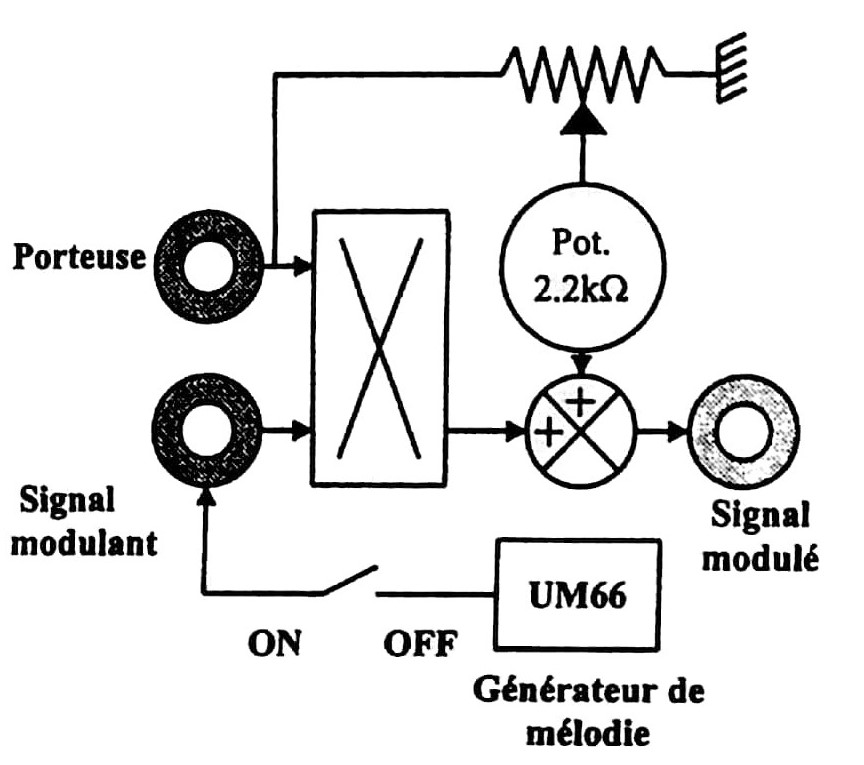
\includegraphics[width=9cm]{modulation}
\end{figure}
L'équation caractéristique de ce dispositif est 
\begin{eqnarray}
V_{mod} = kV_p(t)V_m(t) + KV_p(t)
\end{eqnarray} 
avec ici $k= \frac{1}{10}$.\\
On multiplie le signal que l'on veut transmettre (de fréquence $f_0$) par une porteuse qui oscille à beaucoup plus haute fréquence ($f_p$). On peut alors observer l'allure du signal envoyé : c'est un signal oscillant à $\omega_p$ et dont l'amplitude est modulée par le signal que l'on souhaite transmettre.\\

Si on fait la FFT du signal modulé à l'oscillo on observe trois pics à $f_p$ et $f_p \pm f_0$ comme attendu.\\

On peut maintenant mesurer le taux de modulation
\begin{eqnarray}
m = \frac{2 \times Amplitude(f_p-f_0)}{Amplitude(f_p)}
\end{eqnarray}
Pour $V_p = 5,93$ V, $f_p=200$ kHz, $V_m = 0,52V$ et $f_0=455$ Hz on trouve $m = 2\frac{0,076}{0,46} = 0,33$\\

Si on représente $U_{mod} = f(U_0)$ on observe un genre de trapèze et on a alors 
\begin{eqnarray}
m = \frac{Y_{max}- Y_{min}}{Y_{max}+Y_{min}} = \frac{\lambda_1}{\lambda_2} \stackrel{ici}{=} \frac{1,20 - 0,63}{1,20+0,63} = 0,31
\end{eqnarray}
associé à l'incertitude 
\begin{eqnarray}
\left(\frac{u(m)}{m}\right)^2 = \left(\frac{u(\lambda_1)}{\lambda_1}\right)^2 + \left(\frac{u(\lambda_2)}{\lambda_2}\right)^2
\end{eqnarray}


\section{Démodulation d'amplitude}
\subsection{Détection de l'enveloppe}
\begin{figure}[h]
	\centering 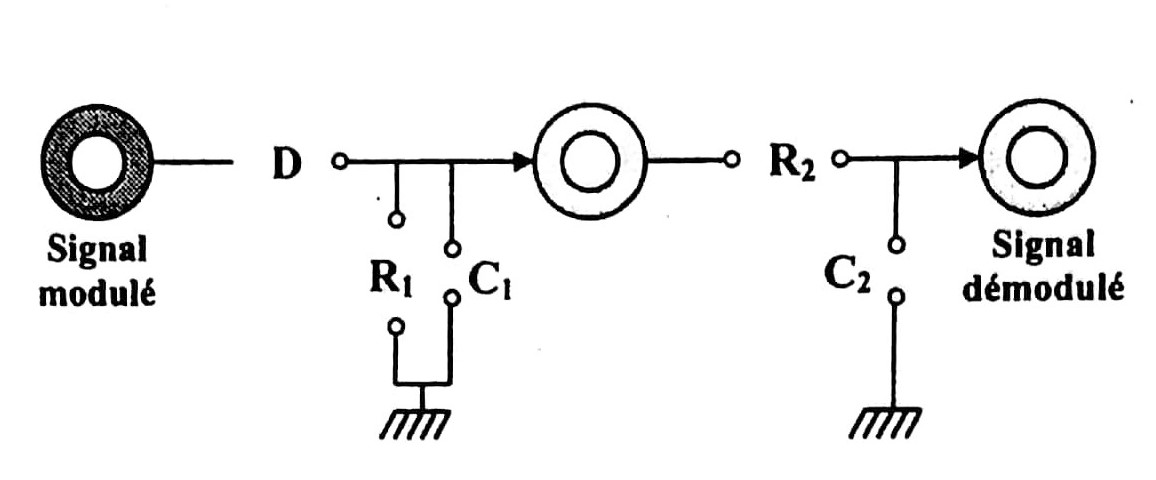
\includegraphics[width=12cm]{enveloppe}
\end{figure}
On mesure la fréquence du signal obtenu en sortie de notre démodulateur et on montre que l'on retrouve bien $f_0$.

\subsection{Détection synchrone}
On regarde cette fois un autre type de détection. On va re-multiplier le signal modulé par la porteuse afin qu'il y ait une harmonique de fréquence $f_0+f_p -f_p = f_0$ : on retrouve ainsi notre signal d'entrée après un filtrage qui enlève les autres fréquences indésirées.
\begin{figure}[h]
	\centering 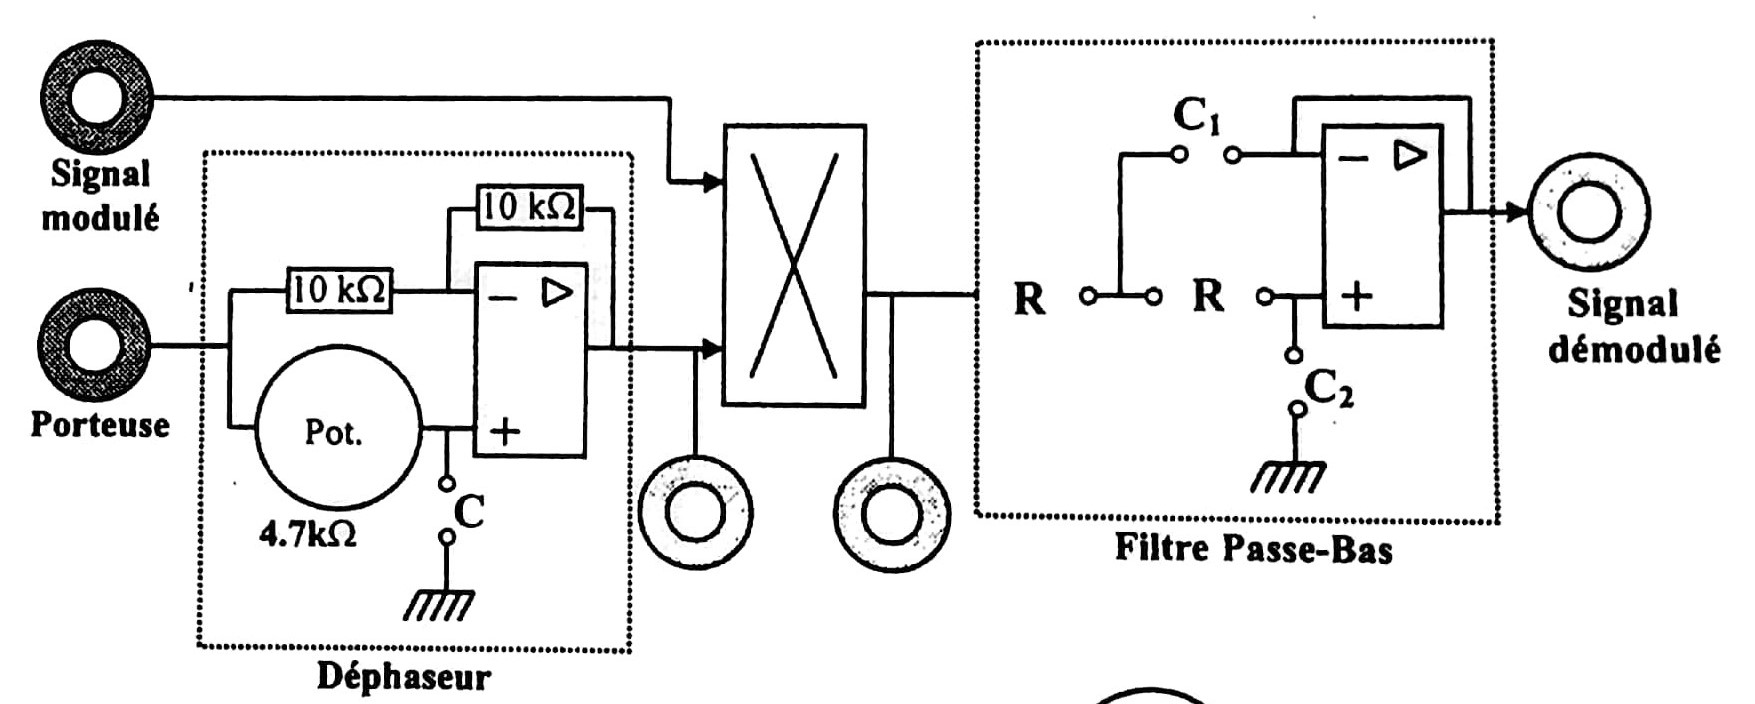
\includegraphics[width=14cm]{detection}
\end{figure}

\section{Câble coaxial}
On envoie un pulse dans un câble coaxial de 50m de long et on mesure le temps que ce pulse met à revenir en se réfléchissant au bout du câble. On en déduit la vitesse de propagation du signal dans le câble.\\

On peut maintenant regarder l'impédance du câble. 

\section*{Questions}
Pourquoi avoir choisi la modulation AM ?\\
Elle est utilisée en radio, et elle possède l'intérêt pédagogique d'être simple.\\

Savez vous comment est constitué un canal stéréo ?\\
On a deux bande : la droite et la gauche (en mode stéréo) que l'on ne peut envoyer en même temps puisqu'ils sont sur la même bande fréquence : il faut donc les moduler.\\
Dans la pratique on transmet les signaux composites : Gauche + Droit à basse frequ et $G-D$ à haute fréquence pour que le signal soit lisible par une chaîne mono aussi (elle aura alors juste le G+D).\\

Quelle est la différence entre fréquence porteuse et débit ?\\
Le débit donne le nombre de bits par seconde, la porteuse nous donne juste la position spectrale du signal.\\

Quelle est la différence entre AM et FM ?\\
En radio FM on est autour de 100 MHz alors que pour l'AM on est autour de 100 kHz. En AM on est plus sensible au bruit qui va venir perturber l'amplitude du signal, en fréquence on aura pas ce problème car une perturbation de l'amplitude n'altère pas l'information. Les spectres du signal émis sont très différents : dans un cas on a 3 pics alors que dans l'autre on a un continuum de fréquences.\\

Qu'est ce que la largeur de fréquence ?
en AM c'est $2f_0$.\\

Comment souhaite t'on que soit cette largeur ? Quelle contrainte cela impose t-il ?\\
faible pour pouvoir transmettre un maximum de signaux (pour plusieurs radio par exemple).\\

Quelle est donc la limitation imposée en radio AM ?\\

Quel est l'intérêt de mesurer le taux de modulation $m$ ?\\
Il faut que $m$ soit inférieur à 1 pour que l'enveloppe du signal ait bien la fréquence $f_0$ (si $m>1$ on détectera une fréquence $2f_0$.\\

Y a t'il une contrainte imposée sur les composantes du RC pour la détection de l'enveloppe du signal ?\\
Oui il faut que l'on ait $\tau_p = 1/f_p \ll RC \ll \tau_m = 1/f_
0$ pour que l'on détecte le signal (on le voit bien en faisant un schéma).\\

Ordre de grandeurs de l'atténuation du câble coax ? Par rapport à la fibre ?\\
20dB par km et 0,2 dB par km pour la fibre (à vérifier).\\

Choix des ampli Op ?\\
On peut comparer les prix et caractéristiques des AOP usuels : 741, TL071 et AD844, on prend le moins cher satisfaisant pour l'utilisation que l'on souhaite en faire, ici un TL072 (deux TL071).
\end{document}